\subsection{Running Python}

\begin{frame}[fragile]
\frametitle{Python console}
To run Python in normal mode, type in a terminal: \\
    \begin{lstlisting}[language=bash, basicstyle=\ttfamily\scriptsize]
python
    \end{lstlisting}
\vspace{-0.5em}
\begin{center}
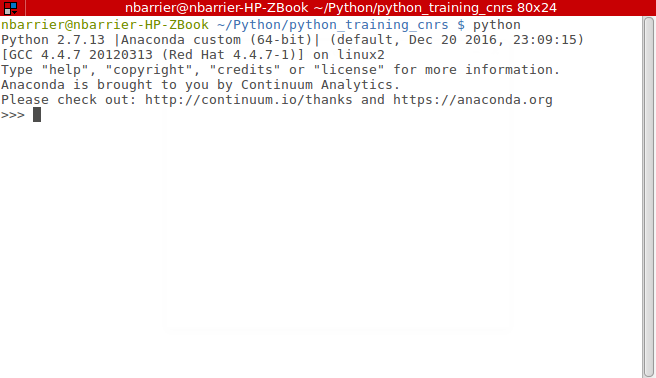
\includegraphics[scale=0.5]{figs/console.png}
\end{center}
\vspace{-2em}
\end{frame}

\begin{frame}[fragile]
\frametitle{Interactive Python}
To run Python in interactive mode, type in a terminal: \\
    \begin{lstlisting}[language=bash, basicstyle=\ttfamily\scriptsize]
ipython 
    \end{lstlisting}
\vspace{-0.5em}
\begin{center}
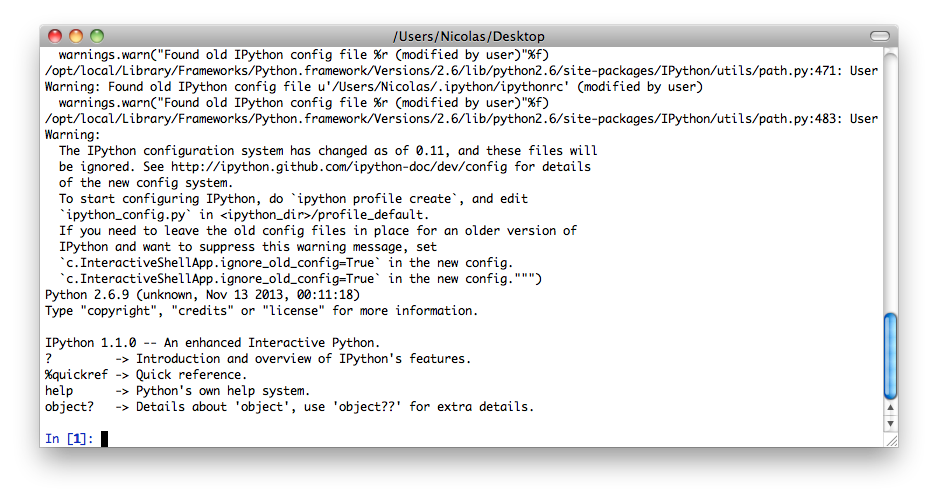
\includegraphics[scale=0.35]{figs/ipython.png}
\end{center}
\vspace{-2em}
%To run a script: \verb+run script.py arg1 arg2 arg3+. \\
%To check your variables: \verb+whos+
\end{frame}

\begin{frame}[fragile]
    \frametitle{Spyder (IDE)}
To run the Python IDE, type in a terminal:\\
\begin{lstlisting}[language=bash, basicstyle=\ttfamily\scriptsize]
spyder &
\end{lstlisting}
\vspace{-0.5em}
\begin{center}
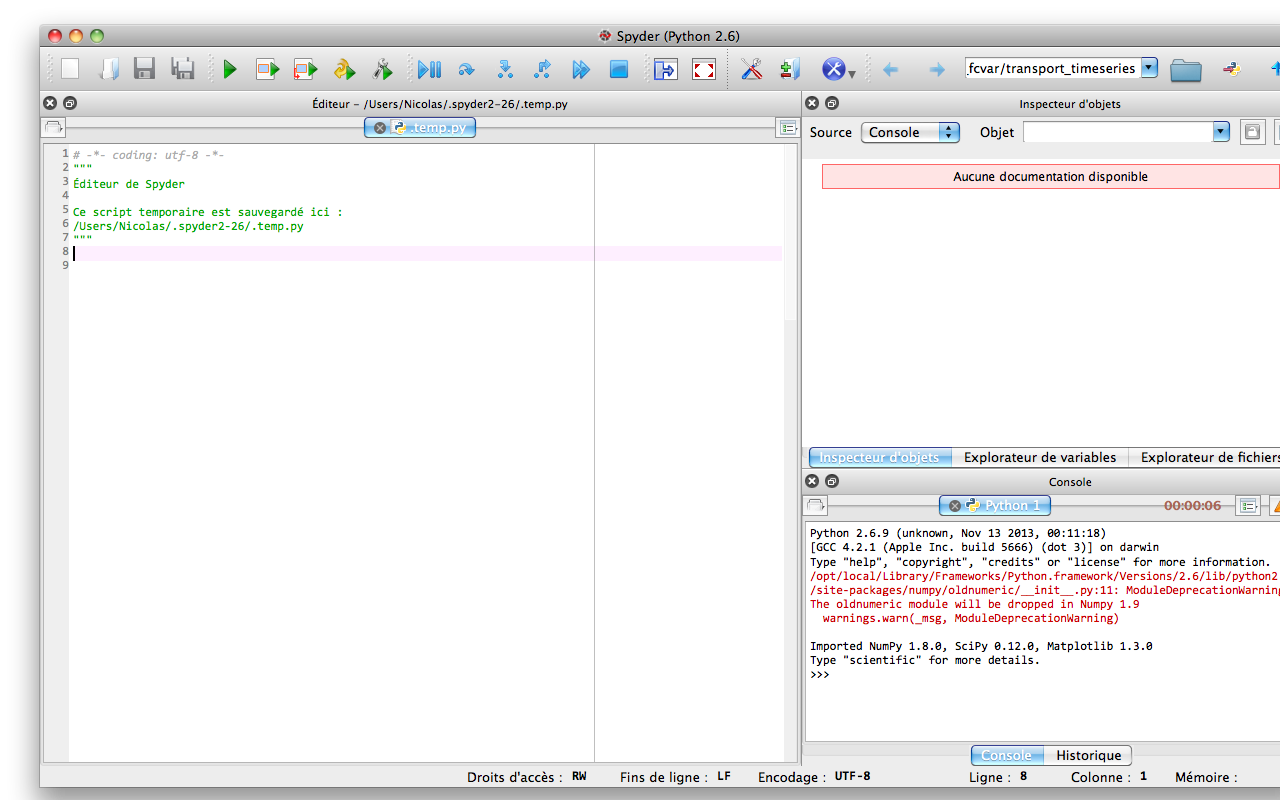
\includegraphics[scale=0.2]{figs/spyder.png}
\end{center}
\end{frame}

\begin{frame}[fragile]
    \frametitle{Jupyter Notebook}
To run the Jupyter Notebook, type in a terminal:
\begin{lstlisting}[language=bash, basicstyle=\ttfamily\scriptsize]
jupyter notebook &
\end{lstlisting}
\vspace{-0.5em}
\begin{center}
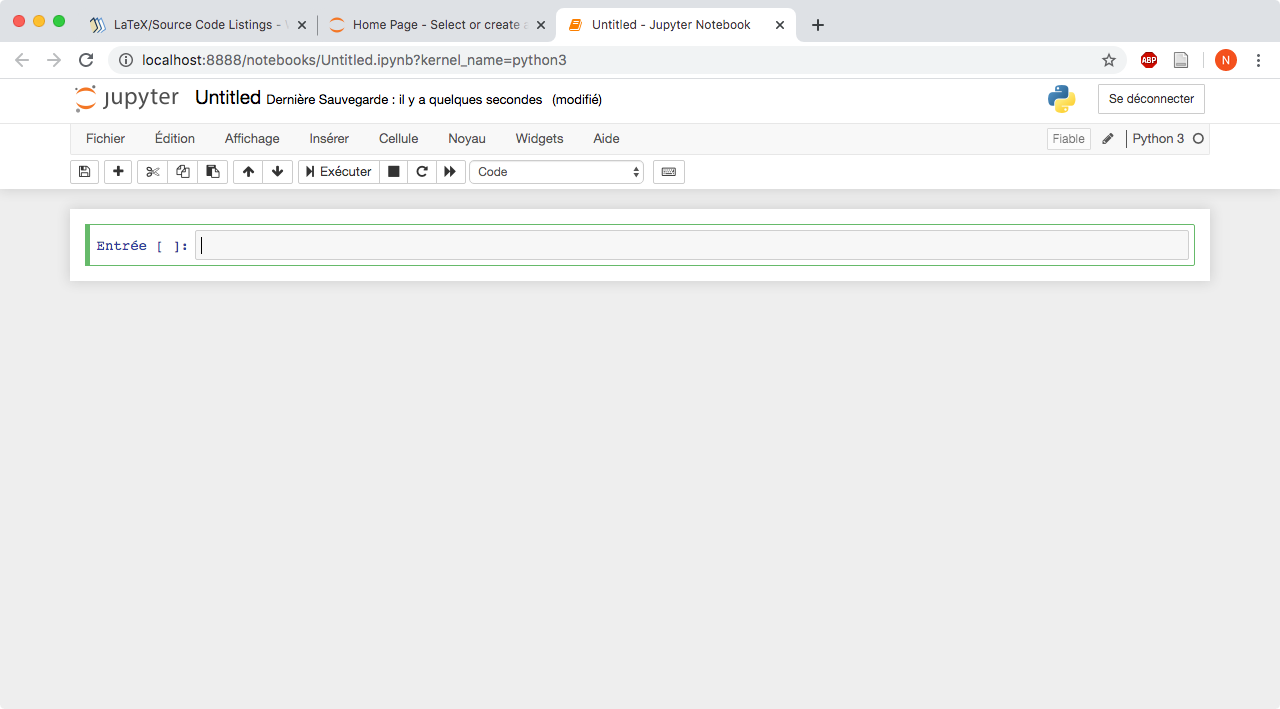
\includegraphics[scale=0.25]{figs/notebook.png}
\end{center}
\end{frame}

\subsection{Running scripts}

\begin{frame}[fragile]
    \frametitle{First script}
    Open a text editor and type in:
    \lstinputlisting[basicstyle=\ttfamily\scriptsize]{scripts/hello.py}
    \vspace{1em}

Save as \verb+hello.py+ and from the terminal type:
    \begin{lstlisting}[language=bash, basicstyle=\ttfamily\scriptsize] 
python hello.py arg1 arg2 arg3
    \end{lstlisting}
    \vspace{0.5em}

You should see:
    \vspace{-0.5em}
    \begin{verbatim}
hello  ['hello.py', 'arg1', 'arg2', 'arg3']
    \end{verbatim}
    \vspace{-1.0em}
    \begin{block}{Note}
The \verb+sys.argv+ statements returns the list of arguments, with the 1st element the name of the script.
    \end{block}
\end{frame}

\begin{frame}[fragile]
    \frametitle{Running from Ipython}
    Open \verb+ipython+ from terminal, then type:
    \begin{lstlisting}[basicstyle=\ttfamily\scriptsize]
run hello.py arg1 arg2 arg3
    \end{lstlisting}
    \vspace{1em}
    To check the environment, type \verb+whos+: 
    \begin{lstlisting}[basicstyle=\ttfamily\scriptsize]
In [2]: whos
Variable   Type      Data/Info
------------------------------
sys        module    <module 'sys' (built-in)>
    \end{lstlisting}
\end{frame}

\begin{frame}[fragile]
    \frametitle{Running from spyder}
    Open \verb+spyder+, open the file and click on the \scriptsize \verb+Run -> Configuration per file+ \normalsize menu. Add arguments to the program as follows:\\
    \vspace{-0.5em}
    \begin{center}
    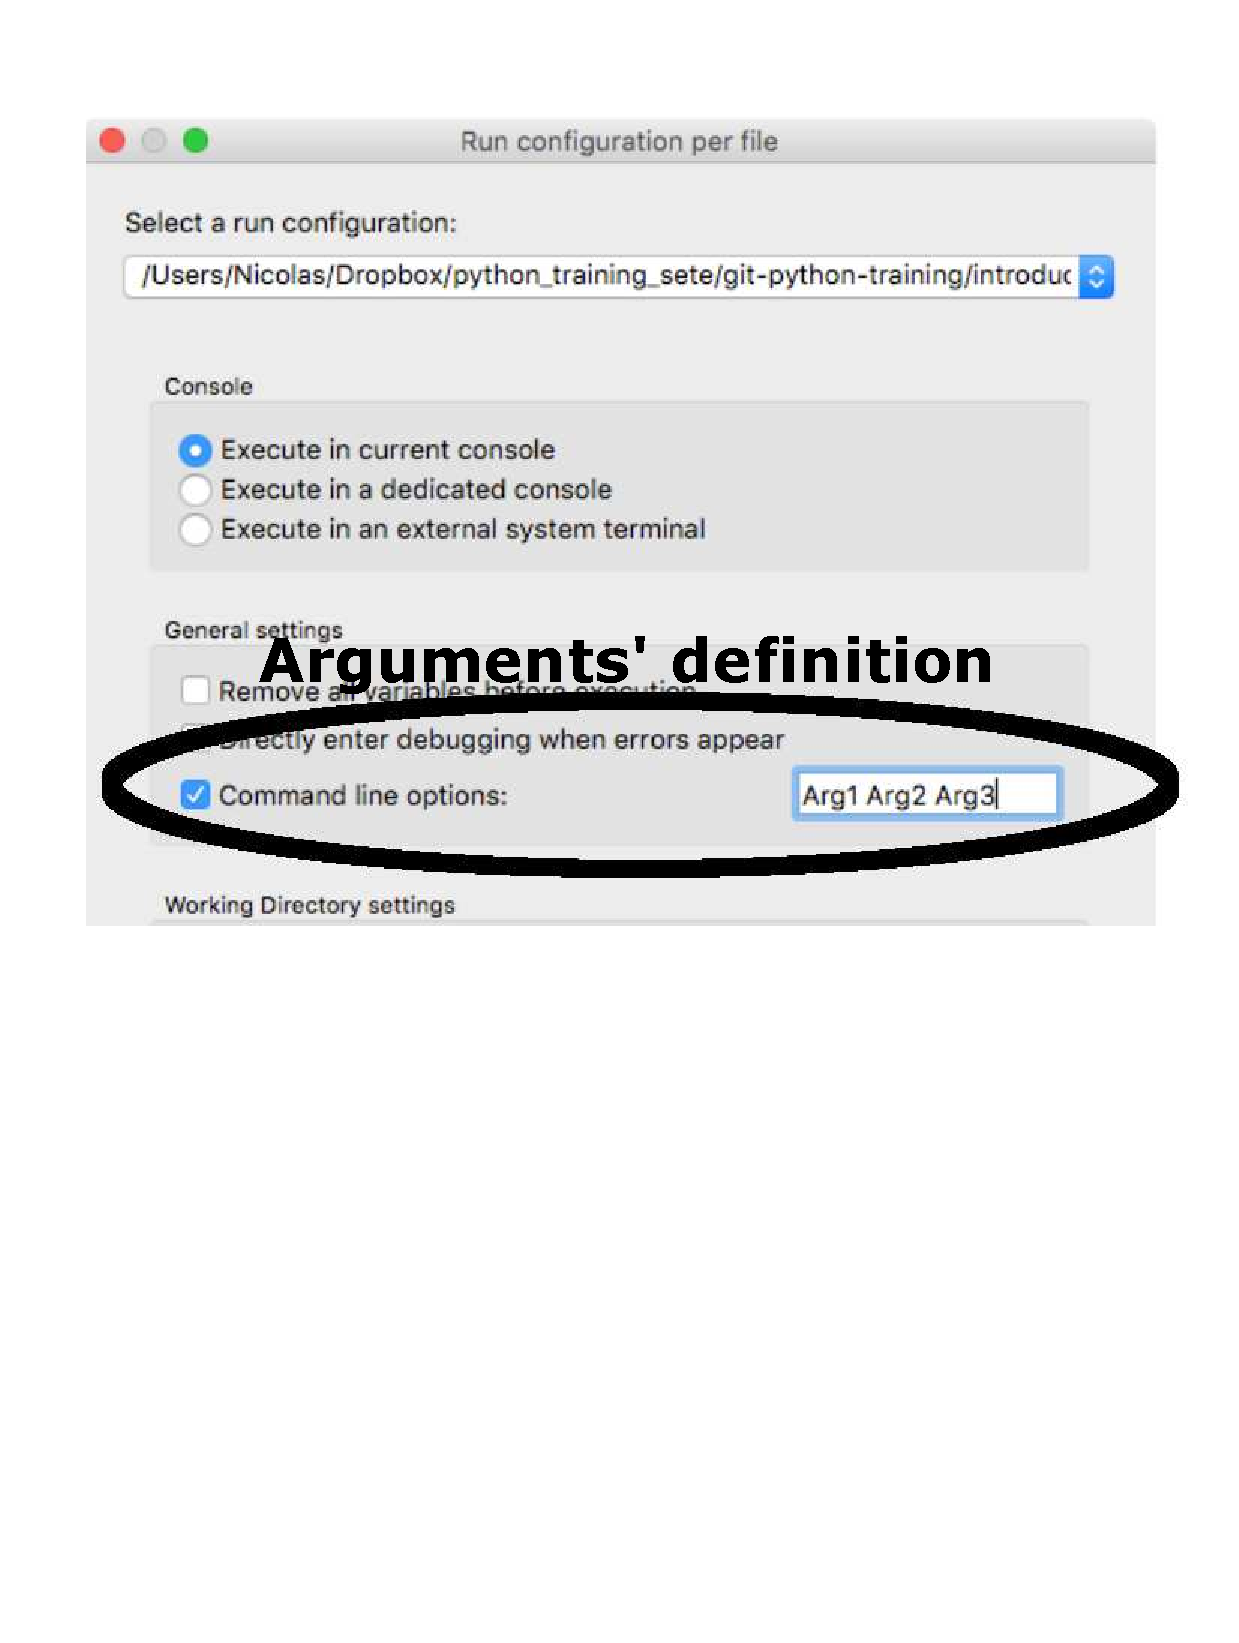
\includegraphics[scale=0.35, trim={0cm 0cm 0cm 0cm}, clip=true]{figs/args_spyder.pdf}
    \end{center}
    Then, click on the \verb+Run file+ button (
\includegraphics[scale=0.5]{figs/run_file.pdf}) to run all the program or the \verb+Run selection+ button
    to run the current line (
\includegraphics[scale=0.5]{figs/run_sel.png}).
\end{frame}
